\section{The reviewed mapping study}

The general topic of the reviewed paper is to conduct an SMS over the topic
of ``Microservices in DevOps''. It should be considered that the context
is specifically set to ``DevOps''. Recent years and recent developments
have risen the attention to the topic significantly. Furthermore, at the
time of writing of the paper, no comprehensive review of the research was
available. Several research questions (RQs) were
asked and afterwards a systematic mapping study (SMS) was conducted upon two
defined search queries. The results were screened and analyzed. Afterwards, the
results were mapped to certain categories and several problems and their solutions
were mapped. After a presentation of the results, a wide discussion of the found
results shows some differences between the theory and effective results \cite{waseem:SMSMSADevOps}.


\subsection{Motivation}

The purpose of the reviewed paper is to create an SMS to understand how 
Microservice Architecture (MSA) is used in conjunction with DevOps \cite{waseem:SMSMSADevOps}.
Furthermore the objective is to identify, analyze and categorize the
existing literature and research around the given topic \cite{waseem:SMSMSADevOps}.
In addition to that, problems and their corresponding solutions - if any - should
be identified \cite{waseem:SMSMSADevOps}. The contribution of the paper to the
academia is a classification of the research, a classification of problems
and their solution, a list of identified research challenges, a classification of
used tools and a list of formal or informal description tools for MSA \cite{waseem:SMSMSADevOps}.


\subsection{Methodology}

With the goal of not limiting the results of such 
an empirical software engineering method to one specific research question,
an SMS is conducted instead of an SLR which provides insight and secondary
data for a particular question \cite{waseem:SMSMSADevOps}. The conducted
SMS was built upon the guidelines that were purposed by Kai Petersen \cite{petersen:SMS}.
The SMS is executed in three steps \cite{waseem:SMSMSADevOps}:

\begin{enumerate}
    \item Planning the mapping study
    \item Collection and analyzing the data
    \item Mapping and documenting the results
\end{enumerate}


\subsection{Research Questions}

Eight different RQs in four categories were derived 
according to the goal of the paper \cite{waseem:SMSMSADevOps}:

~\\
\begin{table}[H]
    \begin{tabularx}{\columnwidth} { 
        | m{0.12\columnwidth} 
        | X | }
        \hline
        \multicolumn{2}{ | X | }{
            Category 1: Demography, classification,
            and mapping of research
        } \\
        \hline
        RQ1.1
        &
        What is the frequency and type of published research
        on MSA in DevOps? \\
        \hline
        RQ1.2
        &
        What are the existing research themes on MSA in
        DevOps and how can they be classified and mapped? \\
        \hline
        \multicolumn{2}{ | X | }{
            Category 2: Problems, solutions, and challenges
        } \\
        \hline
        RQ2.1
        &
        What problems have been reported when implementing
        MSA in DevOps? \\
        \hline
        RQ2.2
        &
        What solutions have been employed to address the
        problems? \\
        \hline
        RQ2.3
        &
        What challenges have been reported when
        implementing MSA in DevOps? \\
        \hline
        \multicolumn{2}{ | X | }{
            Category 3: MSA description methods, patterns,
            and quality attributes
        } \\
        \hline
        RQ3.1
        &
        What methods are used to describe MSA in DevOps? \\
        \hline
        RQ3.2
        &
        What MSA design patterns are used in DevOps? \\
        \hline
        RQ3.3
        &
        What quality attributes are affected when employing
        MSA in DevOps? \\
        \hline
        \multicolumn{2}{ | X | }{
            Category 4: Tool support and application domains
        } \\
        \hline
        RQ4.1
        &
        What tools are available to support MSA in DevOps? \\
        \hline
        RQ4.2
        &
        What are the application domains that employ MSA in
        DevOps? \\
        \hline
    \end{tabularx}
    \caption{Given research questions}
    \label{tbl:RQs}
\end{table}


\subsection{Search}

To collect data, a two-phase-search is used. The first search is applied
to the selected databases with the created search-query. The secondary
search uses a technique called ``snowballing'' \cite{wohlin:Snowballing}. ``Forward snowballing''
includes studies that cite the found studies, while ``backward snowballing''
follows the references of the found research material \cite{wohlin:Snowballing}.

The search is limited to peer-reviewed studies from January 2009 until
July 2018. The starting point was chosen because the term ``DevOps''
was introduced in the year 2009 \cite{waseem:SMSMSADevOps}.

Since MSA has multiple synonyms and can be in context with DevOps or without
the said context, the following two search-strings were compiled \cite{waseem:SMSMSADevOps}:

~\\
\texttt{
((microservi* OR micro-servi*) \\
AND (architect* OR design OR structur*) AND DevOps)
}

~\\
\texttt{(microservice AND DevOps)}

~\\
The search was executed on the following seven databases \cite{waseem:SMSMSADevOps}:

\begin{itemize}
    \item ACM Digital Library (\url{https://dl.acm.org})
    \item IEEE Explore (\url{https://ieeexplore.ieee.org})
    \item Springer Link (\url{https://link.springer.com})
    \item Science Direct (\url{https://www.sciencedirect.com})
    \item Wiley InterScience (\url{https://onlinelibrary.wiley.com})
    \item EI Compendex (\url{https://www.engineeringvillage.com})
    \item ISI Web of Science (\url{https://webofknowledge.com})
\end{itemize}

The execution of the provided search queries on the given databases
yielded a total of 494 studies. After the initial search, the found
studies were screened and categorized into relevant and irrelevant studies.
Of the original 494 studies, only 285 were flagged as ``relevant''.
Those were analyzed according to six generic screening and one specific
screening aspect. After the screening 117 remained flagged as relevant.
Those 117 studies were fully read and scored according to inclusion and
exclusion criteria. At the point when all 117 studies were read and
assessed, 45 studies remained in the relevant category.

In addition to the conducted search, the snowballing technique
yielded additional two studies that should be included in the study.
The results of the snowball were compared with the found results of the
initial search and then the same practices were applied as were on the
initial search.

After the search, a total result of 47 different studies were regarded
as relevant for the SMS \cite{waseem:SMSMSADevOps}.


\subsection{Results}

After the conducted search and the thorough analytical readings and classification
of the 47 studies, the collected results are separated in multiple sections
to answer the RQs given in \autoref{tbl:RQs}:

\begin{itemize}
    \item Demography and classification
    \item Problems, solutions and challenges
    \item Description methods, patterns and quality attributes
    \item Tools and application domain
\end{itemize}


\subsubsection{Demography and Classification}

This subsection should tackle RQ1.1 and RQ1.2 of \autoref{tbl:RQs}.

The conducted search had a year span from 2009 to 2018 \cite{waseem:SMSMSADevOps}.
Despite the broad search parameters of nearly considering a decade worth
of publications, all of the relevant publications were published between
2015 and 2018. The following graph should give some insight into the yearly
publication rate and the type of publication:

\begin{figure}
    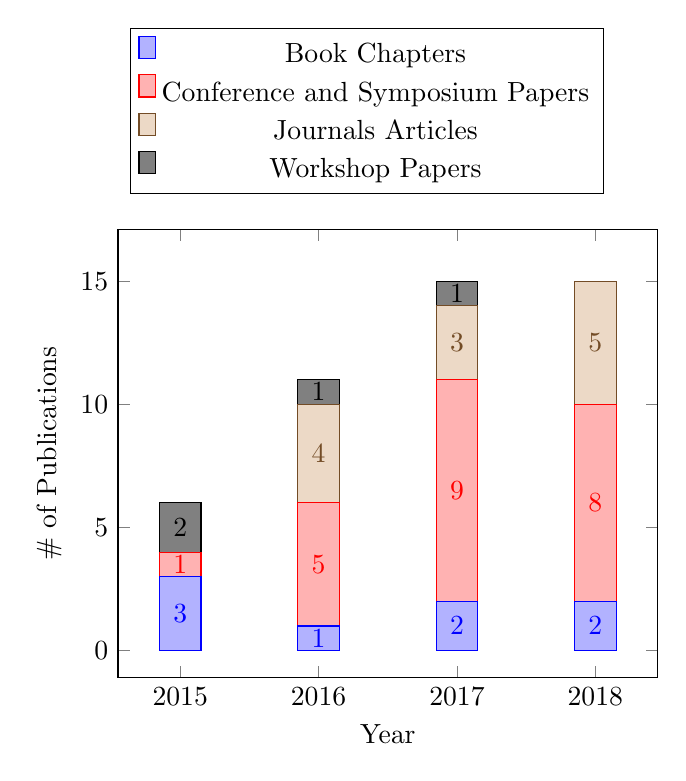
\begin{tikzpicture}
        \begin{axis}[
            ybar stacked,
            bar width=15pt,
            nodes near coords,
            enlargelimits=0.15,
            legend style={
                cells={align=left},
                at={(0.9,1.45)}
            },
            ylabel={\# of Publications},
            xlabel={Year},
            symbolic x coords={2015, 2016, 2017, 2018},
            xtick=data,
            x tick label style={anchor=north},
        ]
            \addplot+[ybar] plot coordinates {
                (2015,3)
                (2016,1)
                (2017,2)
                (2018,2)
            };
            \addplot+[ybar] plot coordinates {
                (2015,1)
                (2016,5)
                (2017,9)
                (2018,8)
            };
            \addplot+[ybar] plot coordinates {
                (2015,0)
                (2016,4)
                (2017,3)
                (2018,5)
            };
            \addplot+[ybar] plot coordinates {
                (2015,2)
                (2016,1)
                (2017,1)
                (2018,0)
            };
            \legend{
                \strut Book Chapters,
                \strut Conference and Symposium Papers,
                \strut Journals Articles,
                \strut Workshop Papers
            }
        \end{axis}
    \end{tikzpicture}
    \caption{Publication activity}
\end{figure}

The distribution of publications over the years gives a detailed intuition
about the general interest of researchers in the specified topic. As seen
in the diagram above, the topic grew more important over the years 2017 and
2018. Since the first publications in 2015 there is an upward trend to
the number of publications \cite{waseem:SMSMSADevOps}.

As for the publication types, over those four years, 23 studies
were published in conference proceedings, 12 in journals, 8 in book chapters
and merely 4 as workshop papers \cite{waseem:SMSMSADevOps}.

The 47 considered papers were all published in 41 venues. The venues
themselves can be devided into four different categories. 17 of the 41
venues count towards the topic \textbf{Internet, Cloud, and Services Computing}.
Another 16 are categorizes as \textbf{Software Engineering} venues. The remaining
8 are split evenly between \textbf{Telecommunications and Networks} with 4 venues
and \textbf{Multi-Disciplinary computing} also with 4 venues \cite{waseem:SMSMSADevOps}.

As for RQ1.2, the result shows, that top two subtopics of the publications
are \textit{Approaches} (13 studies) and \textit{Tools} (12 studies).
The least discussed topic, with only 4 studies, is \textit{Monitoring}
of microservices \cite{waseem:SMSMSADevOps}.


\subsubsection{Problems, Solutions, and Challenges}

During the SMS, with the aid of a thematic analysis on the
extracted data, a total of 24 problems could be identified.
There exist several problems that could not be mapped with a documented
solution so they represent challenges that need further investigation
to provide the community with possibilities to resolve the problem.

The following list should give a brief overview of the identified
problems \cite{waseem:SMSMSADevOps}:

\begin{itemize}
    \item Performance Issue due to Lack of Dedicated Access
    to the Host's Hardware
    \item Empowering Developers through Intelligent Software
    \item Performance Overhead due to Fine Grain Decomposition
    \item Scaling MSA-based Systems
    \item Security and Privacy Across Cloud-Native Applications
    \item Providing Flexible Authentication to Each DevOps Team
    \item Application Decomposition into Microservices
    \item Reducing the Uncertainty in MSA
    \item Managing and Migration Legacy Databases
    \item Modification and Integration of New Functionality in Existing
    Microservices
    \item Operational and Configuration Complexity
    \item Testing of MSA-based Systems in DevOps
    \item Frequent Deployment in Different Environments
    \item Complexity in the Dynamic Deployment
    \item Deployment of MSA-based SaaS at Fine Granular Level
    \item Automatic Optimal Deployment of MSA-based Systems
    \item Logging and Post-Deployment Monitoring
    \item Monitoring and Execution of the Adaptive Actions
    \item Establishing and Maintaining Monitoring Infrastructure
    \item Monitoring Microservices at Run Time
    \item Introducing DevOps and MSA Culture
    \item People Resistance to Adopting DevOps and Microservices
    \item Less Familiarity with Implementing DevOps
    \item Resource management for Development, Deployment,
    and Maintenance of the Cloud-Native Systems
\end{itemize}

For the shown list of problems, at least one solution was provided
in some considered publication which can be viewed in ``Figure 6''
of the reviewed study. In general, a purposed idea to tackle multiple
of the problems is to try not to decompose microservice applications
too fine-grain \cite{waseem:SMSMSADevOps}. As for the general problem
category of ``designing MSA based systems'' multiple solutions are provided.
Many different architectures are promoted and evaluated \cite{waseem:SMSMSADevOps}.

To implement MSA based systems in a DevOps context, many studies suggest
automated pipelines as well as automatic testing libraries. For communicating
with other services, agnostic technologies should be used (like REST over HTTP)
to negate the need of knowledge of a specific programming language 
\cite{waseem:SMSMSADevOps}.

Testing MSA based applications and systems should, according to the considered
papers, be tackled with the given testing strategies that are in place
right now. Which means ``unit testing'', ``integration testing'',
``regression testing'', among others \cite{waseem:SMSMSADevOps}.

The topic of deploying MSA based systems is covered mostly by containerization
and tools like ``Docker Compose'' and ``Kubernetes'' \cite{waseem:SMSMSADevOps}.

Monitoring is purposed to be addressed with frameworks like 
``Unicorn''\footnote{\url{https://www.technative.io/unicorn-framework-the-rise-of-devops-as-a-service/}}
and patter-based approaches like Omnia\footnote{Elaborated in \cite{miglerina:Omnia}}.
The general goal should be, that each team that owns the microservice should be enabled
to monitor their responsibilities \cite{waseem:SMSMSADevOps}.

Problems that relate to culture, people, cost, and other organizational
topics are purposed to be dealt with guidelines for adopting to
new structures in organizations. Cross-functional teams should be introduces
and they should receive training to spread the acceptance of the
new technology \cite{waseem:SMSMSADevOps}.

As for the topic of resource management problems, some considered
studies proclaim to use virtualized or containerized approaches
and well established platforms to share the workspace among
the developers \cite{waseem:SMSMSADevOps}.

~\\
On the contrary, three challenges were identified which
remained unresolved by the papers that were accounted for \cite{waseem:SMSMSADevOps}:

\begin{itemize}
    \item Performance issues due to frequent communication
    \item Providing security at runtime
    \item Generating runtime architectural models
\end{itemize}

Performance issues can emerge when using too fine-grain microservices
or when using synchronous communication channels to other services.

Studies found that security tends to be neglected in general which leads 
to severe vulnerabilities at runtime for microservice based architectures.

Generating models for MSA systems at runtime seems to be an unresearched
topic but could be needed to help with decision-making processes in
adaptive system development.


\subsubsection{MSA descriptions methods, patterns, and quality attributes}

The topic of the third category of RQs orbits around descriptive methods
of MSA systems. What methods and patterns are used and which
quality attributes they should suffice. The regarded studies provided
different patterns and methodologies to describe their architectures
and systems. To summarize the found description methods, five categories
emerged \cite{waseem:SMSMSADevOps}:

\begin{enumerate}
    \item Boxes and Lines (without any "framework")
    \item Unified Modeling Language (UML)
    \item Formal method (e.g. $\pi$-Calculus or equivalent)
    \item Architecture Description Language (ADL)
    \item Others
\end{enumerate}

Out of the 47 studies, 46 used some kind of description.
The distribution is show in the following diagram:

\begin{figure}[H]
    \begin{tikzpicture}
        \pie [rotate = 180]{
            69.5/Boxes and Lines,
            13/UML,
            8/Formal method,
            6.5/ADL,
            3/Others
        }
    \end{tikzpicture}
    \caption{Distribution of descriptive methods}
\end{figure}

To achieve microservice architecture in complex systems, a multitude of
patterns are purposed over all studies. The SMS identified 38 different design
patterns across all regarded papers. The following list should give a brief
overview over the top three recurring patterns \cite{waseem:SMSMSADevOps}:

\begin{enumerate}
    \item Circuit Breaker (5 studies)
    \item Migration pattern (4 studies)
    \item Observer pattern (2 studies)
\end{enumerate}

Regarding affected quality attributes when using MSA in the DevOps context,
the presence of said quality attributes (QA) was confirmed by the SMS.
The QAs were split into two sections, one for positively influenced QAs when
using microservices and one for the negative influenced ones \cite{waseem:SMSMSADevOps}.

\textbf{Positive}
The studies listed the following QAs as being positively influenced:
\begin{itemize}
    \item Deployability (42 studies)
    \item Scalability (32 studies)
    \item Performance (26 studies)
    \item Maintainability (27 studies)
    \item Monitoring (23 studies)
    \item Testability (22 studies)
    \item Flexibility (20 studies)
    \item Availability (19 studies)
    \item Efficiency (19 studies)
    \item Security (10 studies)
    \item Portability (6 studies)
    \item Compatibility (5 studies)
    \item Modifiability (5 studies)
    \item Usability (1 study)
\end{itemize}

\textbf{Negative}
Some studies listed the following QAs as being negatively influenced:
\begin{itemize}
    \item Security (11 studies)
    \item Performance (9 studies)
    \item Scalability (2 studies)
    \item Reliability (2 studies)
    \item Availability (1 study)
    \item Compatibility (1 study)
    \item Maintainability (1 study)
    \item Modifiability (1 study)
    \item Usability (1 study)
\end{itemize}

To have a view from positively mentioned against negatively mentioned,
consider the following chart:

\begin{figure}[H]
    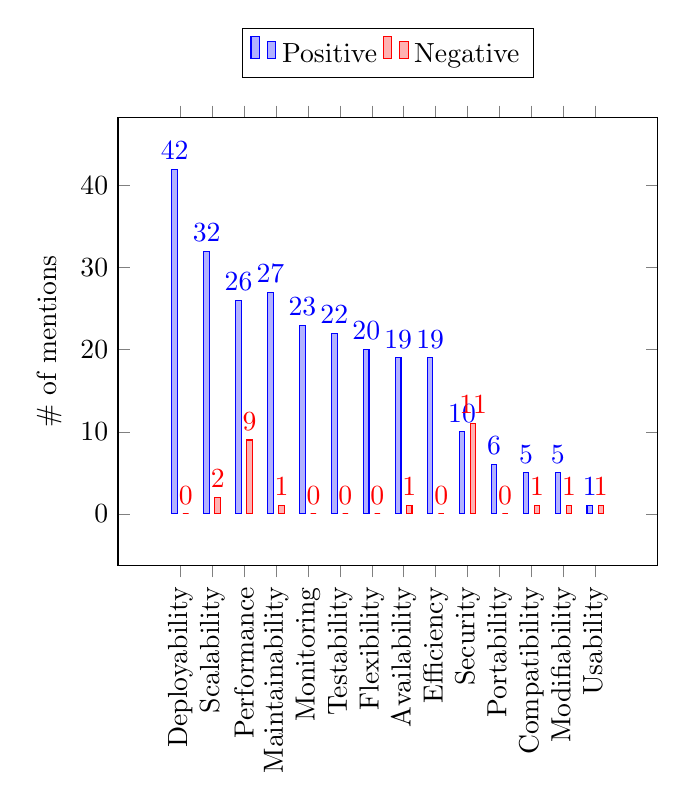
\begin{tikzpicture}
        \begin{axis}[
            ybar,
            bar width=2pt,
            enlargelimits=0.15,
            legend style={
                at={(0.5,1.2)},
                anchor=north,legend columns=-1
            },
            ylabel={\# of mentions},
            symbolic x coords={
                Deployability,
                Scalability,
                Performance,
                Maintainability,
                Monitoring,
                Testability,
                Flexibility,
                Availability,
                Efficiency,
                Security,
                Portability,
                Compatibility,
                Modifiability,
                Usability
            },
            xtick=data,
            x tick label style={rotate=90,anchor=east},
            nodes near coords,
            nodes near coords align={vertical},
        ]
            \addplot coordinates {
                (Deployability,42)
                (Scalability,32)
                (Performance,26)
                (Maintainability,27)
                (Monitoring,23)
                (Testability,22)
                (Flexibility,20)
                (Availability,19)
                (Efficiency,19)
                (Security,10)
                (Portability,6)
                (Compatibility,5)
                (Modifiability,5)
                (Usability,1)
            };
            \addplot coordinates {
                (Deployability,0)
                (Scalability,2)
                (Performance,9)
                (Maintainability,1)
                (Monitoring,0)
                (Testability,0)
                (Flexibility,0)
                (Availability,1)
                (Efficiency,0)
                (Security,11)
                (Portability,0)
                (Compatibility,1)
                (Modifiability,1)
                (Usability,1)
            };
            \legend{
                \strut Positive,
                \strut Negative
            }
        \end{axis}
    \end{tikzpicture}
    \caption{Influenced Quality Attributes}
\end{figure}


\subsubsection{Tool support and application domains}

The fourth category of research questions regards tooling support
and given application domains. The SMS identified 50 different tools and
11 application domains.

The various tools can be seen in Fig. 7 in the SMS \cite{waseem:SMSMSADevOps}.
They were categorized in the following list:

\begin{itemize}
    \item Security Services and Tools (14 tools)
    \item Monitoring Tools (11 tools)
    \item Continuous Integration Tools (7 tools)
    \item Testing Tools (6 tools)
    \item Configuration Management Tools (5 tools)
    \item Build Tools (5 tools)
    \item Version Control Tools (2 tools)
\end{itemize}

The last RQ that is to be answered, is which application domains
exploit the combination of MSA with DevOps. The SMS pinpointed nine
application domains with analyzation of the systems and topics
in the regarded studies. The given domains are stated below \cite{waseem:SMSMSADevOps}.

\begin{itemize}
    \item Not Mentioned
    \item Software Development Tools and Framework
    \item Telecommunication
    \item Mobile Software
    \item E-Commerce system
    \item Embedded system
    \item Financial software
    \item Healthcare software
    \item Webserver
    \item Distributed system
    \item Others
\end{itemize}


\subsection{Discussion}

The following sections will summarize the ``Discussion'' of the SMS. The study
analyzed the found results and explained certain trends.

\subsubsection{Research status and themes}

The limitation of the search to peer-reviewed literature from January 2009 to
July 2018 is based on the ``creation'' of the terms MSA and DevOps.
But the rise of papers and studies followed seven years later, around January 2016.
The study noticed, that 41 papers were published from January 2016 until July 2018
\cite{waseem:SMSMSADevOps}.

As seen in the systematic classification of the research themes, the most recurring
topics are ``Tools'' with 13 studies, ``Approaches'' with 12 studies and
``Development and Deployment'' with 12 studies. This indicates, that the research
is not only centered around new tools, but also regards development life-cycles
as well. On the other hand, there were no publications found that focus on
the topic of ``Requirements Engineering'', be it practices or any other
activities \cite{waseem:SMSMSADevOps}.

\subsubsection{Problems and solutions}

The given solutions in the regarded publications consist, of
design patterns, guidelines, frameworks, etc. For example,
Domain Driven Design (DDD) and Model View Controller (MVC) patterns
are recommended for decomposing an application into a microservice oriented
system. The SMS also states that there are no studies found that
address testing strategies for MSA based systems. As for optimal deployment
of MSA, a very popular solution is the usage of containerization and Kubernetes
\cite{waseem:SMSMSADevOps}.

\subsubsection{Challenges}

A big concern in several papers is performance of such MSA based systems.
The impact can be due to frequent communication between microservices.
Also, poorly engineered architectures can lead to wide spreaded requests
across the whole system. Also, when containers are used, the hardware underneath
has a high impact on performance. The study shows that Amazon EC2 containers are
worse than applications deployed on Amazon EC2 VMs \cite{waseem:SMSMSADevOps}.

The second topic that gets addressed a lot is security. When just ``translating''
applications to MSA, most of the time, security concerns arise. MSA based systems
create complex access control scenarios without any matured patterns to harden
the systems against attackers \cite{waseem:SMSMSADevOps}.

\subsubsection{Description methods and MSA design patterns}

Most studies use just plain, informal boxes and lines as well as UML to
describe microservice architectures. Other methods, like formal $\pi$-Calculator
among others, are used rarely. The SMS argues, that this could be adressed with
the creation of a standard description method for describing MSA
\cite{waseem:SMSMSADevOps}.

The used design patterns are shown in the corresponding table in the SMS.
The most observed pattern is the ``Circuit Breaker'' pattern which indicates,
that cascading failures are a major concern. Next in line is the ``Migration
Pattern'' that recommends various best practices for the transition from
a monolytic application to a MSA based system.
A not so well covered topic are patterns and recommendations
that support CI/CD in MSA \cite{waseem:SMSMSADevOps}.

\subsubsection{Application domains}

The SMS observed, that a third of the studies did not provide a specific application
domain, nor any information to which domain they may count. The rest of the publications
could be categorized into different application domains. The most referenced domain
is ``Software Development Tools and Framework''. This results indicate, that MSA
in the DevOps context is not bound to a specific application domain but rather is
an improvement to a broad range of application domains such as healthcare, finance sector
and embedded systems \cite{waseem:SMSMSADevOps}.
